\section{Evaluation}\label{sec:agg-creds/eval}

The performance of the credential system is evaluated via the instantiation over
pairing-friendly groups. The scheme is instantiated using the
BLS12-381 pairing system. The construction relies only on the bilinearity of the pairing system, 
and so can easily be instantiated with other pairing systems.

We implement the credential system in Go using the \texttt{gnark-crypto}
library~\cite{gnark-crypto}, which provides optimised implementations of group
and pairing operations for BLS12-381. Benchmarks were collected on a MacBook Pro
with an M1 Pro chip and 16GB of RAM.

To assess efficiency, we benchmark the cost of the presentation and verification 
algorithms while first
varying the total number of attributes $n$, and then holding $n$ constant and varying the number of
selectively revealed attributes $k$.  Figures~\ref{fig:agg-creds/vary-n} and
\ref{fig:agg-creds/vary-k} display the results.

The presentation procedure consists of two phases: setup captures the user
preparing commitments to all $n$ attributes, which is independent of $k$, and
proving captures the user generating proofs corresponding to the $k$ revealed
attributes.  We report these phases separately, as they capture distinct costs:
setup grows with $n$, while proving scales with $k$.  Verification also depends
primarily on the number of revealed attributes.

\begin{figure}[h] \centering 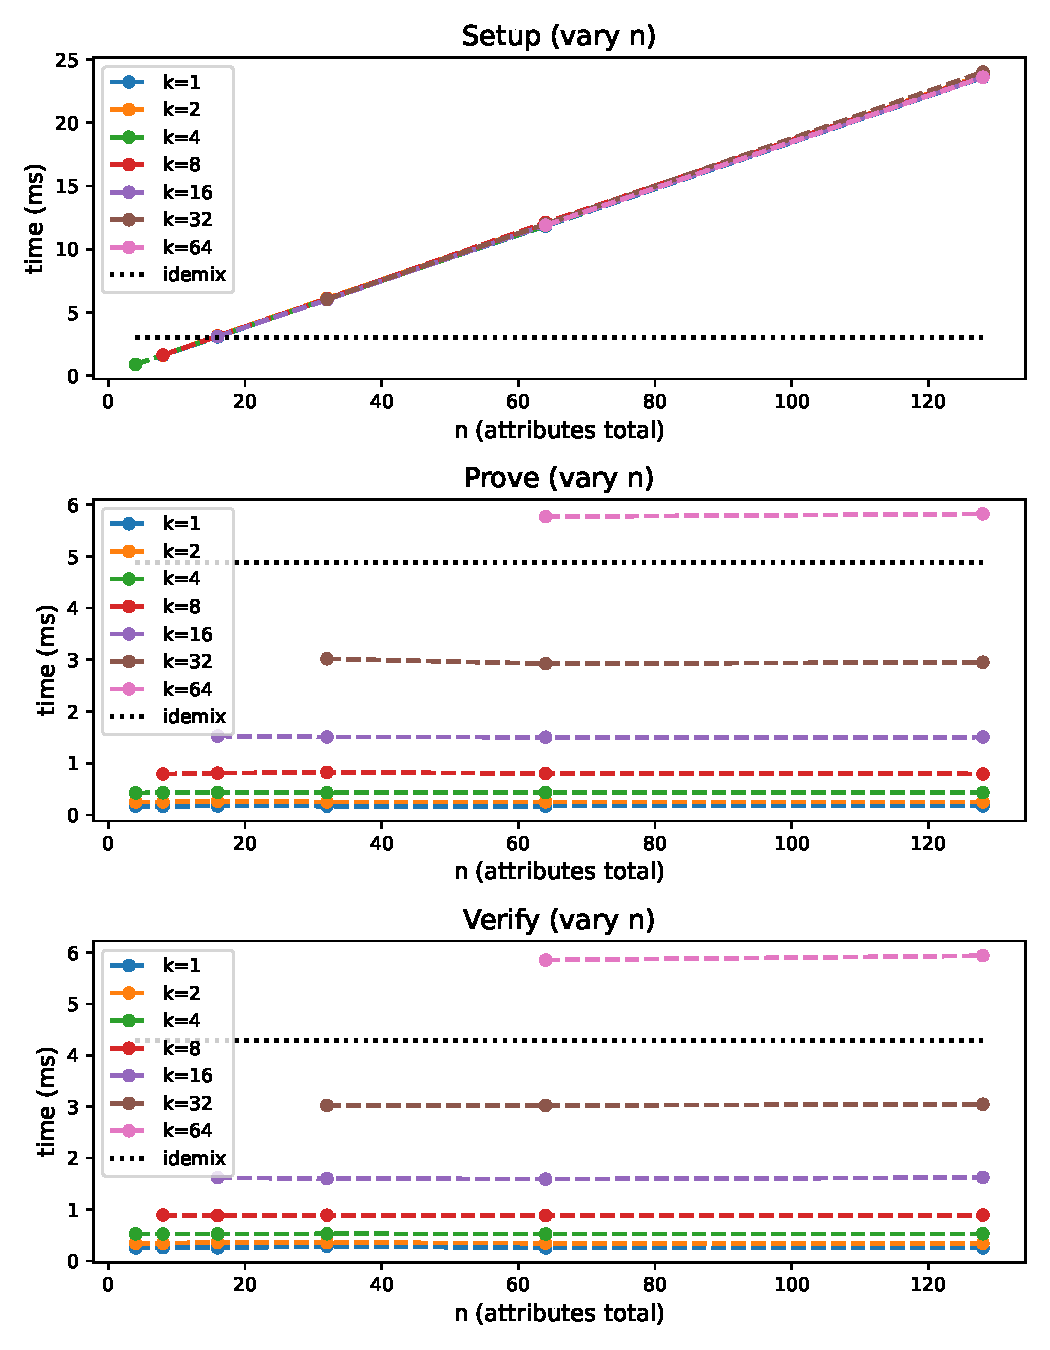
\includegraphics[width=1\textwidth]{chapters/03-agg-creds/vary_n_big.pdf}
\caption{Scaling of setup, proving, and verification with total attributes $n$
varying, for fixed $k$.} \label{fig:agg-creds/vary-n} \end{figure}

\begin{figure}[h] \centering 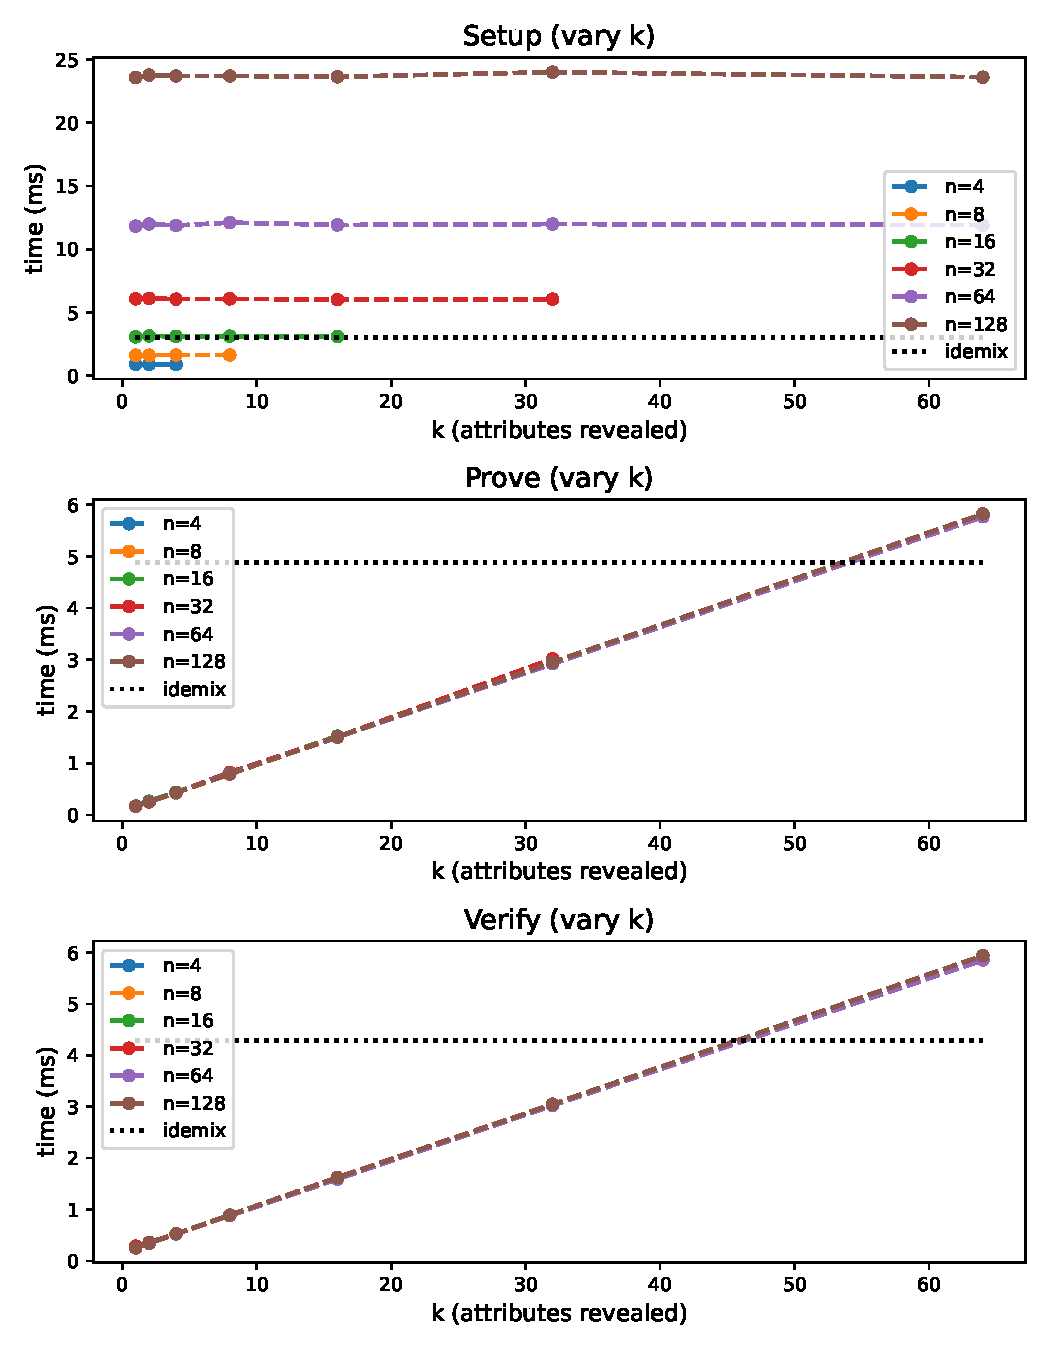
\includegraphics[width=1\textwidth]{chapters/03-agg-creds/vary_k_big.pdf}
\caption{Scaling of setup, proving, and verification with revealed attributes
$k$ varying, for fixed $n$.} \label{fig:agg-creds/vary-k} \end{figure}

Even for $n = 128$ attributes with $k = 64$ selectively revealed, both proving
and verification complete in under $10$ms on a laptop. Setup scales linearly
with $n$, while proving and verification scale linearly with $k$. This
contrasts with credential systems such as Idemix~\cite{CCS:CamVan02}, where proving
and presentation costs depend on the total number of attributes, rather than
the number of disclosed attributes. Overall, our
evaluation demonstrates the practical efficiency of the system: setup and
presentation costs are low enough for client devices, and verification remains
lightweight.